\label{sec:reo}
\section{Introduction}
In the realm of service-oriented programming that is a current trend in software development, the behavior of a software system is not only defined by the functionalities of its underlying services, but also in terms of their interactions. The code written to realize the latter is often referred to as \emph{glue code}. 

Writing and maintaining glue code is a tedious task, especially in complex systems wherein the size and rigidity of the glue code tend to increase over time. This makes these systems hard to modify and maintain. 
Coordination languages offer a more manageable alternative for generating glue code. 

Reo \cite{Arbab04RCC} is a channel-based coordination language for composition of software components and services. Using a small and open-ended set of predefined and user-defined constructs, Reo supports modeling of complex coordination behavior in terms of synchronization, buffering, mutual exclusion, priority, etc. 

The primitive constructs of Reo are \emph{channel}s. Each \emph{channel} has two \emph{end}s, also called \emph{port}s. Channel ends are either of type \emph{source} that read data into the channel or \emph{sink} that write the channel's data out. 

Channels can connect to each other on their ends to form compound elements. Reo \emph{connector}s, also called \emph{network}s are constructed this way. A Reo \emph{node} is formed by one or more channel ends. 

Furthermore, Reo provides a mechanism for hierarchical modeling and abstracting from inner structures by means of \emph{component}s \cite{Arbab04RCC}. A connector can turn into a \emph{component}. In this case it will exhibit (part of) its inner logic as an observable behavioral interface.

Reo emphasizes on the connectors and their compositions rather than the entities that connect to the connectors to coordinate with each others. A Reo connector imposes a specific coordination pattern on interactions occurring between entities. This happens without the entities controlling or being necessarily aware of this pattern. This type of coordination is called \emph{exogenous}, as it is performed from the outside. 

According to a survey of coordination languages \cite{desurvey}, Reo belongs to the class of dataflow-oriented coordination languages, which is between the data-oriented and the control-oriented classes. 

While the main concern of data-oriented coordination languages is consistency among shared data, control-driven languages focus on the flow of control. In comparison, dataflow-oriented languages define the communicating entities, the points of data-flow, and exchanging data-items.

\section{Reo}
In this section, we present an informal overview of the pre-defined set of Reo constructs. %This set includes nodes, a group of channels and three Reo components. 
Following is the list of Reo channels:
\begin{table}[H]
\begin{tabular}{cp{10cm}}
%\hline
       \raisebox{-.1cm}{\sync} & A \emph{sync} channel has a source and a sink end. It accepts data from its source end iff it can dispense it simultaneously through its sink end.
       \\& \\
         \raisebox{-.18cm}{\lossysync} & A \emph{lossySync} has a source and a sink end. It reads a data-item from its source end and writes it simultaneously to its sink end. If the sink end is not ready to accept the data-item, the channel loses it.
\\ & \\
  \raisebox{-.18cm}{\syncdrain} & A \emph{syncDrain} has two source ends and no sink end. It reads data through its two source ends iff both ends are ready to interact simultaneously. The channel discards the received data-items. \\
       \end{tabular}
\end{table}

\begin{table}[H]
\begin{tabular}{cp{10cm}}
  \raisebox{-.18cm}{\syncspout} & A  \emph{syncSpout} has two sink ends and no source end. For each sink end,  the channel generates a data-item out of the underlying data domain  and writes them simultaneously to the corresponding ends.
  \\% & \\
 % \hline
  & \\
  \raisebox{-.2cm}{\asyncdrain} & An \emph{asyncDrain} has two source ends and no sink end. It accepts and discards a data-item from either of its source ends that offers data. If both ends offer data-items simultaneously, the channel chooses one of the ends non-deterministically.     
\\ %& \\% \hline
%\end{tabular}
%\end{table}
%
%\begin{table}[H]
%\centering
%\begin{tabular}{cp{10cm}}
%\hline
& \\ 
\raisebox{-.25cm}{\bcsync} & A \emph{blockSourceSync} channel is a  \emph{Sync} channel that blocks the propagation of priority from its source end toward the sink end. 

This channel and the two next priority blocking channels are used to limit the scope affected by priority, which originates from a \emph{PrioritySync} channel. \\ %& \\ % \hline
& \\
\raisebox{-.23cm}{\bksync} &  A \emph{blockSinkSync}  channel is a  \emph{Sync} channel that stop  spreading of priority from its sink end toward the source end.
\\ %& \\ %\hline
& \\
\raisebox{-.22cm}{\bsync} & A \emph{blockSync}  channel is a combination of \emph{BlockSourceSync} and \emph{BlockSinkSync}. It stops the propagation of priority in both directions.\\
%& \\
%\hline
\end{tabular}
\end{table}

The following is a list of pre-defined Reo components that are abstracted connectors. 

\begin{table}[H]
\centering
\begin{tabular}{cp{10cm}}
%\hline 
%& \\
 \raisebox{-.2cm}{\replicatorNode} & A \emph{replicator} has one source end and one or more sink ends. It replicates data-items coming from its source to its sink ends simultaneously. \\
 & \\
%\hline
%& \\
\raisebox{-.2cm}{\mergerNode} & A \emph{merger} has one or more source ends and a sink end. It chooses one of its source ends that is ready to communicate in a non-deterministic way, receives the incoming data-item, and  writes it to its sink end simultaneously.
\\ & \\
%\hline
%& \\
\raisebox{-.2cm}{\routerNode} & A \emph{router} has one source end and one or more sink ends. It accepts a data-item from its source end and simultaneously replicates it on one of its sink end that is non-deterministically chosen from its set of sink ends, which are ready to accept data. \\
& \\ 
\raisebox{-.2cm}{{\joinNodeWithTweeineenout}}  & A \emph{cross-product} has one or more source ends and a sink end. It accepts a data-item from each of its source ends. Furthermore, it forms a tuple of the data-items that are set in the counter-clock-wise order with respect to the sink node. It writes the tuple on its sink end. All of these operations occur simultaneously. 
\\% & \\
%z\hline
\end{tabular}
\label{table:aa}
\end{table}

%%%Figure ??? shows the original connector corresponding to each component.

As mentioned, Reo nodes are created from channel ends. In case that the node only consists of source ends, it is called a \emph{source} node. A node is \emph{sink}, if it is formed by merely sink ends. Otherwise, if a mixture of source and sink ends collide, the created node is called a \emph{mixed} node.

%A  connector uses source nodes for receiving data from the coordinating entities that are connected to it. Sink nodes are used for writing output to the coordinating entities.  

%A source node acts like a synchronous \emph{replicator} by replicating incoming data-items from its source to its sink ends simultaneously.  

 A mixed node is an atomic combination of a replicator and a non-deterministic merger. Each read and write action needs all of its involved source and sink ends to be able to interact synchronously. Otherwise, the action cannot take place.

\section{Examples}
%Followings are few Reo networks  that are used throughout the thesis. 
%
\begin{BehExample}
 Figure \ref{fig:reoex1} shows a Reo network that is composed of a \emph{lossySync} and a \emph{FIFO$_1$} channel. When the \emph{FIFO$_1$} channel is empty, the \emph{lossySync} reads a value from its source end and passes it to its sink end that coincides with the source end of the \emph{FIFO$_1$} channel. Therefore, the \emph{FIFO$_1$} channel becomes full. The data stored in the \emph{FIFO$_1$} channel can be read and consumed via its sink channel. Before that the \emph{FIFO$_1$} channel loses its data, the  \emph{lossySync} channel accepts but loses all its incoming data. % to the \emph{lossySync} are lost by it.

\begin{figure}[!ht]
\centering
\mesallossyfif
\caption{An example of a context-dependent Reo network}
\label{fig:reoex1}
\end{figure}
\end{BehExample}

\begin{BehExample}
Figure \ref{fig:reoex2} depicts a Reo network consisting of two \emph{filter} channels with negating conditions. The first channel reads a data item from its source end and writes it on its sink end if it matches its condition, otherwise it loses the data. In the former case, the data item will not satisfy the condition corresponding to the second channel, so it is lost by the second channel. In both cases, there won't be any write operation on the sink end of the second channel. 

\begin{figure}[!h]
\centering
\mesaldofilter
\caption{An example of a data-aware Reo network}
\label{fig:reoex2}
\end{figure}
\end{BehExample}

\begin{BehExample}
Figure \ref{fig:reo2} illustrates a Reo network containing two \emph{FIFO$_1$} channels. The network behaves as a \emph{FIFO$_2$} buffer. In the beginning, both channels are empty. If there is an incoming data item on the source end of the first channel, the channel accepts the data and becomes full. Then, by an internal transition the data item is moved to the second channel. It makes it possible for the first channel to read another data item and/or to writes out the stored data through the sink end of the second channel.

 \begin{figure}[!ht] 
   \centering
      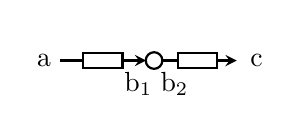
\begin{tikzpicture}[>=stealth]
      \draw (-.8,0) node [thin]{a};
    %  \draw [->,thick,dashed] (-.3,0) -- ++(.8,0);
      \draw ++(.6,.3) node [thin]{};
      \draw ++(.4,-.3) node [thin]{b$_1$\ };
      \draw ++(.8,-.3) node [thin]{\ b$_2$};
      \draw [thick] (.6,0) circle (3pt);
      \draw ++(.75,.25) node [thin]{};%c
      \draw ++(1.9,0) node [thin]{c};
      \draw [thick](0.7,0) -- (.9,0);
      \def\rectanglepath{-- ++(0, .1) -- ++(.5,0) -- ++(0,-.2) -- ++(-.5, 0) -- ++(0,.1) --cycle}
      \draw [thick] (-.3,0) \rectanglepath;
 \draw [thick](-.6,0) -- (-.3,0);
 \draw [->,thick] (.2,0) --++(.3,0);
      \draw [thick] (.9,0) \rectanglepath;
      \draw [->,thick] (1.4,0) --++(.25,0);
    \end{tikzpicture}
    \caption{A Reo network for a FIFO$_2$ buffer}
    \label{fig:reo2}
   \end{figure}      
\end{BehExample}

\section{Extensible Coordination Tools (ECT)}
A variety of Reo related tools are bundled together in a common framework, called Extensible Coordination Tools (ECT) \cite{ect}. The tools in the framework are integrated as Eclipse plugins and operate based on the operational semantics of Reo, most notably, connector coloring and variations of constraint automata. ECT includes tools to design, transform, animate, model check, test, perform QoS analysis, and generate executable code from Reo connectors. 

%The followings are out contribution to ECT framework in the context of this thesis:
%\begin{itemize}
%\item BPEL to Reo Converter
%\item UML SD to Reo Converter 
%\item UML AD to Reo Converter
%\item The BPMN 2 to Reo converter plugin,
%\item A constraint-based framework to calculate operational semantics of Reo with respect to various formal semantics of Reo,   
%\item A tool to support priority and propagation of priority in a Reo connector.
%\end{itemize}

%Figure \ref{fig:} shows 
The ECT tools can be chained together to enable analysis on business process models.  
%, which are developed over yeas by researchers working on Reo.
%\subsection{ECT plugins}
%Several tools developed over years by researchers working on Reo have been integrated into ECT. Here is a brief overview of
%them. 
%\begin{figure}[ht]
%    \centering
%    \caption{An example of BPMN2 transaction}
%    \label{fig:emfreo}
%\end{figure}
Here, we briefly overview these tools: 

\begin{itemize}
\item \emph{Graphical editor}: 
The graphical editor provides facilities to design Reo networks. The editor has been implemented based on the Eclipse Modeling Framework (EMF) \cite{emf} and Eclipse Graphical Modeling Framework (GMF).
As a requirement of the model-driven approach and to work with EMF, Reo meta-model has been defined in \cite{Krause11a} \cite{Krause201123}. 
%Figure \ref{fig:emfreo} illustrates the core of the Reo meta-model.
%
%. The shown classes and interfaces are part
%of the package cwi.reo. For brevity, multiplicities of associations are omitted if they
%are 0..1. In the following, we explain the Reo meta-model in detail.
\item \emph{Animation tool}:
 The animation tool produces simulation of Reo networks in the format of Adobe Flash \cite{flash}. The tool is based on the animation semantics introduced in  \cite{davidtez} and
 visualizes the token game in Reo connectors  \cite{Krause11a}.

\item \emph{Verification tool}: %Rephrase TODO
 Vereofy \cite{vereofypaper} is a model checker for Reo networks developed at the Technical University of Dresden. It can be used independently or from the ECT.

\item \emph{mCRL2 conversion tool}: 
 Another model checker for Reo networks that is integrated into ECT is the mCRL2 \cite{mcrl2}.
The mCRL2 to Reo converter tool translates constraint automata specifications of Reo into mCRL2 specifications.% in the mCRL2 specification language. It supports data, context-dependency and time.

\item \emph{Execution engines}: ECT includes two execution engines:  i) The centralized execution engine of Reo is a code generation framework based on constrained automata \cite{BaierCA}. ii) The distributed execution engine for Reo is implemented based on constraint-based semantics of Reo \cite{JoseThesis}.
%Alternatively, Jos\'{e} Proen\c{c}a \cite{JoseThesis} has implemented a distributed execution engine for Reo networks.

\item \emph{The Extensible Automata (EA) framework}: 
 Extensible Automata (EA) framework is a unified framework for generating automata-based semantics of Reo networks. The framework comes with a graphical automata editor, which also can be used outside of the context of Reo. It includes functionality to generate automata models with stochastic information from
graphical Reo models. From these models, it is possible to extract Continuous Time Markov Chains (CTMCs) that can be analyzed by the external tools such as PRISM probabilistic model checker \cite{Kwiatkowska} or ECT stochastic simulation tool \cite{oscarmaster}.

\item \emph{BPMN 2 to Reo conversion tool}: 
In the context of this thesis, we have implemented a plugin to convert BPMN 2 models into Reo connectors \cite{behnaz}. The converter deals with transactions, whose behavior is relatively more complex to map, in a two phases manner. 

The first phase is refinement, wherein transactions are substituted by a group of BPMN 2 elements, which collectively presents the same behavior as the transaction, yet they are easier to be mapped to Reo.  In the second phase, the BPMN 2 constructs are being matched against some patterns to generate corresponding Reo elements. Chapter \ref{ch:mapping} elaborates on the converter. %, we presented the implementation of the ECT converter plugin, which automates the transformation of %BPMN, BPEL and UML 2 Sequence Diagram to Reo
% Reo conversion tools have been used for capturing formal semantics of high-level modeling languages, namely, 
%BPEL, 
%BPMN2, and UML2. In our work \cite{behnaz}, we presented the implementation of the ECT converter plugin, which automates the transformation of %BPMN, BPEL and UML 2 Sequence Diagram to Reo. 

\item \emph{Constraint-based semantics calculator}: As part of this thesis, we have implemented a tool to generate data-dependent, context-sensitive, and priority-aware formal semantics of Reo. To generate the automata-based formal semantics of Reo networks, we express the behavior of the Reo network in term of constraint satisfaction problem. From the solutions to this problem, we build the automata model. 

Our approach in using constraint solving to get the semantics of a Reo network is similar to the one used to generate the distributed execution engine for Reo \cite{ClarkeProenca10}. However, unlike \cite{ClarkeProenca10} \cite{JoseThesis} , we support data, time, and priority. Another difference is that we calculate the all the possible behavior, while the mentioned tool has a step-wise approach that find the next possible behavior at a time.  In Chapter \ref{chapterCASM}, we present our approach in details. 

Our work is the first tool support for priority in Reo. Chapter \ref{ch:prio} elaborates on our approach in obtaining a priority-aware formal semantics of Reo from the solutions of constraints generated from each of Reo elements in a compositional manner.
\end{itemize}

%In chapter \ref{ch:mapping}, we present our implementation of BPMN 2.0 to Reo converter. The BPEL to Reo transformer is a considerable refinement and enhancement  of the first version of the converter that has been developed at the University of Tehran. As it was erroneous and inefficient because of its failure in composing different parts of Reo networks. It also lacks abstraction.  Furthermore, we improve the implementation of UML SDs to Reo, which is originally developed at the University of Leiden. Unlike the original implementation, where the diagrams were written manually in the text format, our implementation accepts the models exported in XMI %TODO
%format from graphical UML design tools.
%After such a transformation, refined and annotated Reo process models can be visualized, verified and transformed into executable code with the help of the Eclipse Coordination Tools (ECT)~\cite{}.
%\cite{behnaz}The conversion of 
%therefore contains conversion tools from various modeling languages to Reo. Most importantly,
%conversion from BPEL, BPMN2, and UML2 sequence diagrams is supported.
%For more information we refer to [24].
%
%
 %In this paper, we solely consider UML SDs among UML diagrams. 
 %Transformation of the UML Activity Diagrams can be performed similarly to that of BPMN and is not discussed here. Our focus on these notations is primarily due to their exploitation in the EU COMPAS project\footnote{http://www.compas-ict.eu/} for the design of business process fragments. Process fragments in this context can be understood as design patterns for the implementation of service-based systems compliant to relevant legislation and organizational policies.????
%
%We provide the first implementation for the BPMN to Reo conversion, and a considerably refined implementation of the BPEL to Reo converter. The first version of the latter converter, developed at the University of Tehran, was erroneous and inefficient due to its failure to compose different parts of Reo networks and the absence of abstraction.
%TODO rephrase
%GOOD TODO Graphical representation of process models in Reo helps us to trace the errors discovered using model checking tools back to the source models. This would not be possible if we assumed direct conversion to automata-based models or process algebras. The architecture of the ECT converters  is shown in Figures~\ref{fig:} and \ref{fig:arch}. 
%
%\begin{figure}
%  \centering
  %\sub figure[An overview of the ECT converters ]{
%    \includegraphics[width=.99\textwidth]{img/}
  %  \vspace{-4mm}
 % \caption{Application of our converters????}
  %    \label{fig:}
%\end{figure}
%
%\begin{figure}
%  \centering
%  %\sub figure[ECT converters  architecture]{
%%\vspace{-4mm}
%  \caption{ECT converters }
%      \label{fig:arch}
%\end{figure}
%
%TODO rephrase
%\begin{figure}
%  \centering
%      \begin{tikzpicture}[>=stealth]
%       \filldraw [black] (0,0) circle (1pt) (0.5,0) circle (1pt) (1,0) circle (1pt) (3,0) circle (1pt) (3.5,0) circle (1pt)
%                         (0.5, -0.7) circle (1pt) (1,-0.7) circle (1pt) (3,-0.7) circle (1pt) (3,-0.7) circle (1pt);
%       \draw (0,0.3) node {write};
%       \draw (3.5,0.3)  node {read};
%       \draw [->, thick]  (0,0) -- (0.5,0);
%       \draw [->, thick]  (0.5,0) -- (1,0);
%       \draw (1,-0.3) rectangle (3, 0.3);
%       \draw (2,0)  node[font=\itshape] {ShiftLossy};
%       \draw (1,-1) rectangle (3, -0.4);
%       \draw (2,-0.7)  node[font=\itshape] {ShiftLossy};
%       \draw [->, thick]  (3.0,0) -- (3.5, 0);
%       \draw [->, thick]  (3.5, 0) -- (3.5, -0.7);
%       \draw [->, thick]  (3.5,-0.7) -- (3, -0.7);
%       \draw [-, thick]  (1,-0.7) -- (0.5, -0.7);
%       \draw [->, thick]  (0.5,-0.7) -- (0.5, 0);
%       \draw [-, thick]  (0,0) -- (0, -1.2);
%       \draw [-, thick]  (0,-1.2) -- (3.5, -1.2);
%       \draw [->, thick]  (3.5, -1.2) -- (3.5, -0.7);
%       \draw (3.5, -0.7) circle (1pt);
%    \end{tikzpicture}
%%\vspace{-8mm}
%  \caption{Variable}	
%  \label{fig:bpelvar}
%%\vspace{-4mm}
%\end{figure}

%\begin{figure}[ht]
%  \centering
%    \begin{tikzpicture}[>=stealth]
%       \filldraw [black] (0,0) circle (1pt) (1,0) circle (1pt) (2.3, 0) circle (1pt)
%                         (0, -1) circle (1pt) (1,-1) circle (1pt) (1.6,0) circle (1pt);
%       \draw (0,0.3) node {in};
%       \draw (2.3,0.3)  node {out};
%       \draw [->, thick]  (0,0) -- (0.5,0);
%       \draw [->, thick]  (1,0) -- (0.5,0);
%       \draw [-, thick]  (0,0) -- (0, -0.25);
%       \draw (-0.1,-0.25) rectangle (0.1, -0.7);
%       \draw [->, thick]  (0,-0.7) -- (0, -1);
%       \draw [-, thick]  (0,-1) -- (0.25, -1);
%       \draw (0.25,-1.1) rectangle (0.7, -0.9);
%       \draw [->, thick]  (0.7, -1) -- (1, -1);
%       \draw [-, thick]  (2.3, 0) -- (1.85, 0);
%       \draw (1.85,-0.1) rectangle (1.4, 0.1);
%       \draw [->, thick]  (1.4, 0) -- (1, 0);
%       \draw (1,-1.3) rectangle (2.3, -0.7);
%       \draw (1.6, -1) node[font=\itshape] {Router};
%       \draw [->, thick]  (1.4, -0.7) -- (1, 0);
%       \draw [->, thick]  (1.9, -0.7) -- (2.3,0);
%    \end{tikzpicture}
%%\vspace{-4mm}	
%\caption{Lossyshift}
%\label{fig:lossyShift}
%%\vspace{-4mm}	
%\end{figure}
%
%\begin{figure}[ht]
%  \centering
%    \begin{tikzpicture}[>=stealth]
%       \filldraw [black] (0,0) circle (1pt) (0.5,0) circle (1pt) (1.5,0.5) circle (1pt) (1.5,-0.5) circle (1pt) (1.5,0) circle (1pt) (2,0.5) circle (1pt) (2,-0.5) circle (1pt);
%       \draw [->, thick]  (0,0) -- (0.5,0);
%       \draw [->, dashed] (0.5,0) -- (1.5,0.5);
%       \draw [->, thick]  (1.5,0.5) -- (2, 0.5);
%       \draw [->, dashed] (0.5,0) -- (1.5,-0.5);
%       \draw [->, thick]  (1.5,-0.5) -- (2, -0.5);
%       \draw [->, thick]  (1.5,0.5) -- (1.5,0);
%       \draw [->, thick]  (1.5,-0.5) -- (1.5,0);
%       \draw [->, thick]  (0.5,0) -- (1,0);
%       \draw [->, thick]  (1.5,0) -- (1,0);
%    \end{tikzpicture}
%    \caption{Router}
%\label{fig:router}
%%\vspace{-4mm}	
%%\vspace{-4mm}	
%\end{figure}
%
%\subsection{Supporting Priority}
%\begin{figure}[ht]
%  \centering
%    \begin{tikzpicture}[->,>=stealth',shorten >=1pt,auto,node distance=1.4cm,semithick]
%      \tikzstyle{every state}=[draw=black,text=black,minimum size=10pt]
%      \node[state] (s1) {};
%      \node[state] (s2) [right of=s1] {};
%      \path (s1) edge node {write} (s2)
%            (s2) edge [loop above]  node {write} (s2)
%            (s2) edge [loop below]  node {read} (s2);
%    \end{tikzpicture}
%    \caption{Constraint automata of BPEL variable}
%    \label{fig:cafasl2}
%%\vspace{-4mm}	
%%\vspace{-4mm}	
%\end{figure}
%
%\subsubsection{BPEL to Reo Converter}
%The BPEL2Reo transformer is based on the approach proposed in~\cite{TVM+08}. The main motivation for our work is to resolve problems we discovered in the tool presented in~\cite{TVM+08}. One of the problems is that it generates a number of disjoint nodes in an output Reo model. 
%
%Another problem is
%the large size of the output models for relatively small BPEL structures. For example, the mapping of the widely used BPEL element \textit{variable} leads to a Reo network shown in Figure~\ref{fig:bpelvar}, which consists of two \emph{ShiftLossy} networks shown in Figure~\ref{fig:lossyShift}. Each \emph{ShiftLossy} network, in turn, contains a \emph{Router} connector shown in Figure~\ref{fig:router}. Thus, the mapping of a single BPEL variable produces a network with more than 20 channels, including 6 channels with asynchronous FIFO1 buffers. For any middle-size BPEL specification containing dozens of variables, such a mapping already leads to a state explosion problem. We have resolved this issue by employing components. Thus, rather than dealing with complex connectors, we map some BPEL elements to components whose behavior is described by fairly small constraint automata. Figure~\ref{fig:cafasl2} shows such an automaton for the BPEL variable element. Intuitively, the states of this automaton represent uninitialized and initialized states of a variable: once a value is written to the variable, it can be read infinitely many times, as well as reset to another value written to the source node of the network. In the aforementioned automaton we abstract from the data constraints. However, for enabling data analysis, different values of the variable will correspond to different states of the automaton. The components that correspond to basic BPEL structures such as \textit{variable}, \textit{receive} or \textit{reply} operations are predefined at the design time, and then loaded and placed into a target Reo model at the runtime. Compound structures such as \textit{sequence}, \textit{while} and \textit{pick} are transformed into a set of channels that glue the appropriate basic structures. In this way, we achieve a significant performance optimization compared to the previous version of the tool.
%
%\subsubsection{UML SD to Reo Converter} %TODO rewrite
%Another converter plug-ins within the ECT converter , UML SD to Reo, accepts UML2.x SD models as input and generates a set of Reo networks for representing message exchange between communicating actors. The communication protocols expressed in Reo then can be visualized and verified automatically. This is especially important in the context of case-based development as it allows designers to reason about global communication schemas given the interaction protocols of particular entities.
%
%The initial version of this conversion tool, developed at the University of Leiden, is as a stand-alone program which accepts input files with message sequences in a proprietary text format. This hampers the tool's interoperability with other frameworks, in particular, with UML design toolkits.%, and makes the tool hard to use in practice.
%We modified the converter to enable the transformation of the models generated by a UML2 graphical designing tool called Bouml \cite{bouml} \footnote{At the time of development, BOUML (http://bouml.free.fr/) was the only free UML2 tool we found that supported both Activity Diagrams and XMI format export. Recently Model Development Tools (MDT) project for Eclipse Galileo has provided support for UML2 Activity Diagrams.% Now we are looking forward to a more stable version of MDT to integrate in our .
%} 
%
%The choice of Bouml is justified by the fact that it is a free UML2 tool that runs under all major operating systems and supports the exchange of models via an eXchanging Model Information (XMI) format. XMI aims at providing a standard specification for exchanging model information between tools and repositories. Moreover, each UML2 tool may have its own implementation of XMI. Therefore, the idea of exchanging UML2 models between tools is not yet practical. For this reason, in order to support each UML2 tool, we are required to have a corresponding XMI parser. Figure~\ref{fig:arch} shows XMI parsers of Bouml and Eclipse UML2 tool. The XMI parser parses the input and loads the model into objects that represent the elements of UML SDs (e.g., actors, lifelines, combined fragments, messages). After that, the loaded model is traversed and its elements are translated to Reo connectors. 
%
%\begin{figure}[ht]
%    \centering
%    \caption{An example of BPMN2 transaction}
%    \label{fig:emfreo}
%\end{figure}
